%%%%%%
%
% $Autor: Wings $
% $Datum: 2020-01-18 11:15:45Z $
% $Pfad: WuSt/Skript/Produktspezifikation/powerpoint/ImageProcessing.tex $
% $Version: 4620 $
%
%%%%%%


\chapter{Material List}

In this section it is included additional information, relevant for the project development among other technical, financial and theoretical explanations related to the Digitization of Meter's Digits, with an ESP32-CAM.


\bigskip

%%%%%%%%%%%%%%%%%%%%%%%%%%%%%%%


List of materials required for the project:

\begin{itemize}
    \item \textbf{ESP32-CAM AI-Thinker} 
    
    \begin{itemize}
        \item Description: ESP32-CAM is a low-cost ESP32-based development board with onboard camera (OV2640), small in size. It is an ideal solution for \ac{iot} application, prototypes constructions and \ac{diy} projects. The board integrates WiFi, traditional Bluetooth and low power BLE , with 2 high-performance 32-bit LX6 CPUs.
        \item Link Datasheet: \url{https://media.digikey.com/pdf/Data%20Sheets/DFRobot%20PDFs/DFR0602_Web.pdf}
        \item Cost: Approximately 10 Euro.
    \end{itemize}
    
    \begin{figure}  
        \begin{center}
            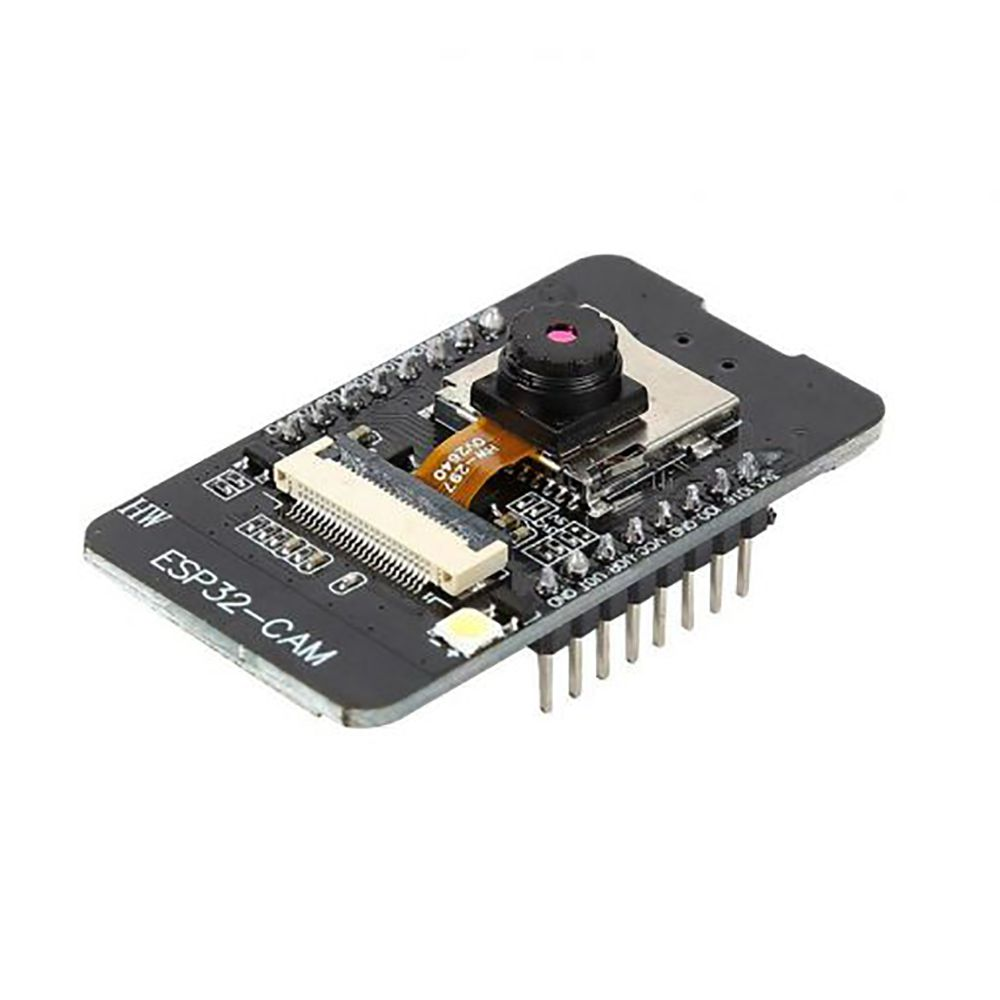
\includegraphics[width=12cm, height=6cm]{ESP32/ListMaterialESP32CAM}
            \caption{ESP32-CAM.} 
            \label{fig:ESP32-CAM.}
            \footnotesize \textbf{Reference:} \cite{Elektor:2022}
        \end{center}
    \end{figure}	
    
    \item\textbf{OV2640 Camera} 
    
    \begin{itemize}
        \item Description: OV2640 Camera is a 2 Megapixel OV2640 camera module with an f3. 6mm lens. It contains a 24pin FPC interface. A wide-angle lens and 1632 x 1232 high resolution make it a perfect camera for Grove AI HAT for Edge Computing and other Sipeed serial board.
        \item Link Datasheet: \url{https://www.uctronics.com/download/cam_module/OV2640DS.pdf}
        \item Cost: Approximately 5 Euro.
    \end{itemize}
    \begin{figure}  
        
        \begin{center}
            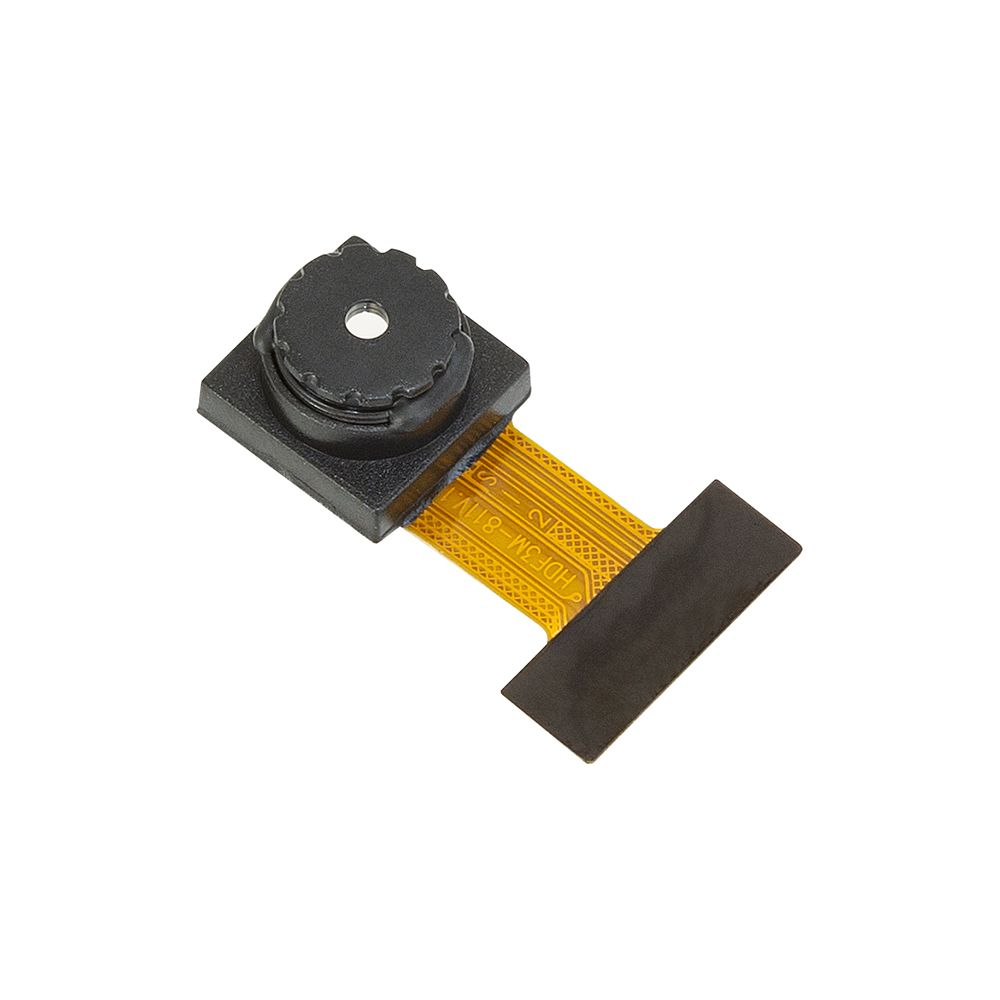
\includegraphics[width=12cm, height=6cm]{ESP32/OV2640}
            \caption{OV2640 Camera.} 
            \label{fig:OV2640 Camera.}
            \footnotesize \textbf{Reference:} \cite{ArduCam:2022}
        \end{center}
    \end{figure}	
    
    \item \textbf{ESP32-CAM-MB USB Programmer} 
    
    \begin{itemize}
        \item Description: The ESP32-CAM AI-Thinker MB programmer is a shield that can be attached to the ESP32-CAM board GPIOs. The programmer comes with the CH340C USB to serial chip; this allows serial communication to the ESP32-CAM using the USB port on the shield. Additionally, the shield also comes with a RESET and a BOOT (IO0) buttons. This may be useful to easily reset the ESP32-CAM or put it into flashing mode.
        \item Link Datasheet: N/A
        \item Cost: Approximately 2 Euro.
    \end{itemize}
    
    \begin{figure}  
        \begin{center}
            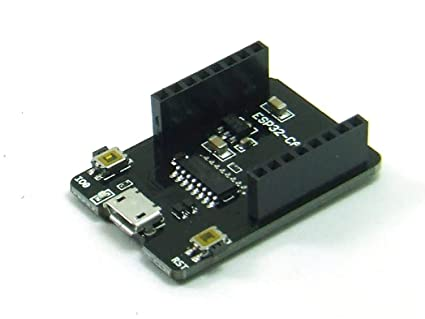
\includegraphics[width=12cm, height=6cm]{ESP32/ListMaterialESP32MB}
            \caption{ESP32-CAM-MB USB Programmer.} 
            \label{fig:ESP32-CAM-MB USB Programmer.}
        \end{center}
    \end{figure}	
    
    \item \textbf{Secure Digital (SD) Card \(16 GB\)} 
    
    \begin{itemize}
        \item Description: A memory Secure Digital card is an electronic data storage device used for storing digital information, typically using flash memory. These are commonly used in digital portable electronic devices. They allow adding memory to such devices using a card in a socket instead of a protruding USB flash drives.
        \item Link Datasheet: \url{https://www.intenso.de/en/products/memory-cards/microsd-card-class-10}
        \item Cost: Approximately 5 Euro.
    \end{itemize}
    \begin{figure}  [H]
        \begin{center}
            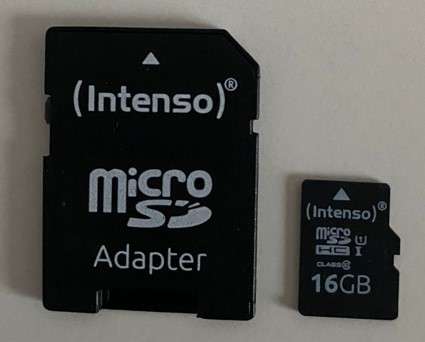
\includegraphics[width=12cm, height=6cm]{ESP32/ListMaterialSDCard}
            \caption{Secure Digital Card.} 
            \label{fig:Secure Digital Card.}
        \end{center}
    \end{figure}	
    
    \item \textbf{ESP32-CAM Case} 
    
    \begin{itemize}
        \item Description: A case to store the ESP32-CAM module to make it easy for the user transportation, install, and handle.
    \end{itemize}
    
    \begin{figure}  
        \begin{center}
            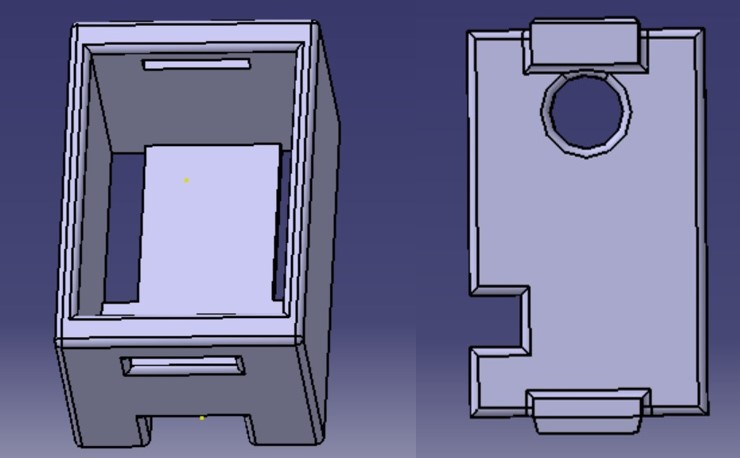
\includegraphics[width=12cm, height=8cm]{ESP32/CamCase}
            \caption{ESP32-CAM Case.} 
            \label{fig:ESP32-CAM Case.}
            \footnotesize \textbf{Reference:} Designed by Author
        \end{center}
    \end{figure}	
    
    \item \textbf{USB cable - USB A / micro USB B}
    
    \begin{itemize}
        \item Description: USB 2.0 cable with A Male to Micro B connectors is a High-Speed Transmission device that supports up to 480 Mbps. It is mostly used for charging Android phones and tablets or connecting \ac{pc} peripherals such as hard drives, printers, and more. In this specific case, to enable the communication between \ac{pc} and ESP32-CAM.
        \item Link Datasheet: \url{https://www.tme.eu/Document/700e9581ffc48a630c6d37ae87e788bc/esb22.pdf}
        \item Cost: Approximately 3 Euro.
    \end{itemize}
    \begin{figure}  
        \begin{center}
            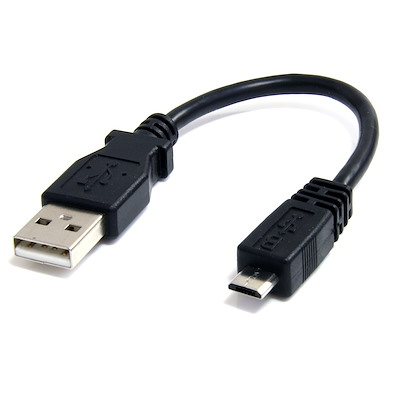
\includegraphics[width=12cm, height=6cm]{ESP32/ListMaterialUSB}
            \caption{USB cable - USB A / micro USB B.} 
            \label{fig:USB cable - USB A / micro USB B.}
        \end{center}
    \end{figure}	
\end{itemize}
\ac{sw} List of materials required for the project:
\begin{itemize}
    \item \textbf{Python v3.10.}
    
    \begin{itemize}
        \item Description: Python is a computer programming language often used to build websites and software, automate tasks, and conduct data analysis. Python is a general-purpose language, meaning it can be used to create a variety of different programs and isn't specialized for any specific problems.
        \item Link Release Notes: \url{https://docs.python.org/3/whatsnew/3.10.html}
        \item Cost: FREE - Open source.
    \end{itemize}
    
    \begin{figure}  
        \begin{center}
            
\includegraphics[width=12cm, height=6cm]{ESP32/ListMaterialPython}
            \caption{Python 3.10.} 
            \label{fig:Python 3.10.}
        \end{center}
    \end{figure}			
    
    \item \textbf{Visual Studio Code v1.73.1.} 
    
    \begin{itemize}
        \item Description: \ac{vscode}, is a source-code editor made by Microsoft with the Electron Framework, for Windows, Linux and macOS. Features include support for debugging, syntax highlighting, intelligent code completion, snippets, code refactoring, and embedded Git.
        \item Link Release Notes: \url{https://code.visualstudio.com/updates/v1_73}
        \item Cost: FREE - Open source.
    \end{itemize}
    \begin{figure}  [H]
        \begin{center}
            
\includegraphics[width=12cm, height=6cm]{ESP32/ListMaterialvscode}
            \caption{Visual Studio Code v1.73.1.} 
            \label{fig:Visual Studio Code v1.73.1.}
        \end{center}
    \end{figure}			
    
    \item \textbf{ESP-IDF \ac{vscode} Plug-In v1.5.1.} 
    
    \begin{itemize}
        \item Description: ESP-IDF is Espressif's official \ac{iot} Development Framework for the ESP32, ESP32-S, ESP32-C and ESP32-H series of SoCs. It provides a self-sufficient SDK for any generic application development on these platforms, using programming languages such as C and C++.
        \item Link Release Notes: \url{https://github.com/espressif/vscode-esp-idf-extension/releases/tag/v1.5.1}
        \item Cost: FREE - Open source.
    \end{itemize}
    \begin{figure}  
        \begin{center}
            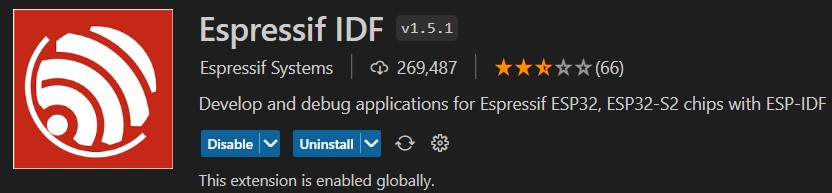
\includegraphics[width=12cm, height=6cm]{ESP32/ListMaterialIDF}
            \caption{ESP-IDF Plug-In v1.5.1.} 
            \label{fig:ESP-IDF Plug-In v1.5.1.}
        \end{center}
    \end{figure}
\end{itemize}

%%%%%%%%%%%%%%%%%%%%%%%%%%%%%%%
%\section{Software Bill Of Materials (SBOM)}

%%%%%%%%%%%%%%%%%%%%%%%%%%%%%%%


